%%%%%%%%%%%%%%%%%%%%%%%%%%%%%%%%%%%%%%%%%%%%%%%%%%%%%%%%%%%%%%%%%%%%%%%%%%%%%%%%
%% Projeto Final de Graduação
%% Aluno: Victor Seixas Souza
%% Orientadora: Christiane Neme Campos
%% Tema: Teoria de Ramsey em Grafos
%%%%%%%%%%%%%%%%%%%%%%%%%%%%%%%%%%%%%%%%%%%%%%%%%%%%%%%%%%%%%%%%%%%%%%%%%%%%%%%%
% !TEX root = ../thesis.tex
%%%%%%%%%%%%%%%%%%%%%%%%%%%%%%%%%%%%%%%%%%%%%%%%%%%%%%%%%%%%%%%%%%%%%%%%%%%%%%%%

\chapter{Números de Ramsey Clássicos}
\label{chap:prelim}

%%%%%%%%%%%%%%%%%%%%%%%%%%%%%%%%%%%%%%%%%%%%%%%%%%%%%%%%%%%%%%%%%%%%%%%%%%%%%%%%

Antes de estudar os números $R(k)$ para valores maiores de $k$, é conveniente generalizar nossas definições. Até agora, definimos os números de Ramsey da seguinte maneira: $R(k)$ é o menor inteiro positivo $n$, tal que qualquer coloração de arestas em duas cores do $K_n$ possui um $K_k$ monocromático. Existem diversas maneiras de generalizar esta definição, a primeira delas está explicitada a seguir.

%%%%%%%%%%%%%%%%%%%%%%%%%%%%%%%%%%%%%%%%
\begin{definition}
$R(k,s)$ é o menor inteiro positivo $n$, tal que qualquer coloração de arestas em duas cores do grafo $K_n$ possui um $K_k$ da primeira cor ou um $K_s$ da segunda cor.
\end{definition}
%%%%%%%%%%%%%%%%%%%%%%%%%%%%%%%%%%%%%%%%

Note que esta definição contém a antiga pois $R(k) = R(k,k)$, que são chamados de \indef{números de Ramsey diagonais}. Ressaltamos que não é preciso demonstrar novamente que estes números estão bem-definidos, uma vez que segue da definição que $R(k,s) \leq R(\max\{k,s\}) < \infty$.

%%%%%%%%%%%%%%%%%%%%%%%%%%%%%%%%%%%%%%%%%%%%%%%%%%%%%%%%%%%%%%%%%%%%%%%%%%%%%%%%

\section{Pequenos Números de Ramsey}

Vamos analisar inicialmente alguns valores de números de Ramsey que são imediatos de determinar. Por exemplo $R(1,k) = 1$ para qualquer valor de $k$, uma vez que é impossível evitar um $K_1$ monocromático em qualquer cor quando o grafo possui vértices. Além disso, temos $R(2,k) = k$, dado que não possuir $K_2$ em alguma cor significa que ela não está presente na coloração. Como temos a simetria $R(k,s) = R(s,k)$, os valores realmente interessantes são obtidos para $k,s \geq 3$; o primeiro deles, $R(3,3) = 6$, já apresentado.

Vamos agora estudar o número $R(3,4)$, utilizando um argumento semelhante ao do $R(3,3)$, porém ligeiramente mais sofisticado. O número $R(3,4)$ foi determinado em 1955, por Greenwood e Gleason~\cite{greenwood}, e está apresentado a seguir. Neste trabalho, os autores obtiveram outros resultados e alguns destes também estão apresentados a seguir.

%%%%%%%%%%%%%%%%%%%%%%%%%%%%%%%%%%%%%%%%
\Needspace*{4\baselineskip}
\begin{proposition}[Greenwood, Gleason~\cite{greenwood}]
\label{prelim:thm:r34}
$R(3,4) \leq 9$.
\end{proposition}
%%%%%%%%%%%%%%%%%%%%%%%%%%%%%%%%%%%%%%%%
\begin{proof}
Seja $G$ um grafo completo com nove vértices e $c$ uma $RB$-coloração.
Suponha que não exista $K_3$ vermelho ou $K_4$ azul. Seja $v \in V(G)$ um vértice qualquer. Considere as vizinhanças $N_R(v)$ e $N_B(v)$ de tamanhos $d_R(v)$ e $d_B(v)$, respectivamente. Assim, temos que $d_R(v) + d_B(v) = 8$. Suponha que $d_R(v) \geq 4$. Se existirem $x,y \in N_R(v)$ tais que $c(xy) = R$, então formamos um triângulo vermelho unindo as extremidades desta aresta com $v$, o que é absurdo. Por outro lado, se esta aresta for azul, temos um $K_4$ azul em $N_R(v)$. Concluímos que $d_R(v) \leq 3$, o que implica $d_B(v) \geq 5$.

Suponha que $d_B(v) \geq 6$. Como sabemos que $R(3,3) = 6$, $N_B(v)$ possui um triângulo monocromático. Como $G$ não possui $K_3$ vermelho, então $N_B(v)$ possui um $K_3$ azul. Contudo, isto nos dá uma contradição, pois unindo este $K_3$ com o vértice $v$, temos um $K_4$ azul. Portanto, podemos concluir que $d_B(v) = 5$ e $d_R(v) = 3$. Isto, no entanto, vale para qualquer vértice de $G$, em particular, implica que $G_R$ possui 9 vértices de grau ímpar.
Entretanto, pelo \emph{handshaking lemma}, sabemos que a quantidade de vértices de grau ímpar em um grafo precisa ser par, e então chegamos num absurdo.

Portanto, em qualquer caso, contradizemos a hipótese de que não existe $K_3$ vermelho ou $K_4$ azul e, assim, concluímos que $R(3,4) \leq 9$.
\end{proof}
%%%%%%%%%%%%%%%%%%%%%%%%%%%%%%%%%%%%%%%%

%%%%%%%%%%%%%%%%%%%%%%%%%%%%%%%%%%%%%%%%
\begin{figure}[ht!]
\centering
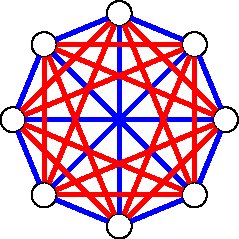
\includegraphics{figures/2_prelim_1_r34lb}
\caption{Coloração de arestas do $K_8$ sem $K_4$ vermelho e sem $K_3$ azul.}
\label{prelim:fig:exr34}
\end{figure}
%%%%%%%%%%%%%%%%%%%%%%%%%%%%%%%%%%%%%%%%

A Proposição~\ref{prelim:thm:r34} estabelece uma cota superior para $R(3,4)$. Uma forma de obter uma cota inferir é por meio da construção de uma coloração de arestas em duas cores de um grafo completo sem $K_3$ vermelho e sem $K_4$ azul.
A Figura~\ref{prelim:fig:exr34} exibe uma tal coloração com 8 vértices. Isto implica que $R(3,4) > 8$, que em conjunto com a Proposição~\ref{prelim:thm:r34}, implica que $R(3,4) = 9$. Embora apenas evidenciar uma coloração seja suficiente, existem $2^{\binom{8}{2}} = 2^{28} = 268435456$ colorações de arestas do $K_8$ em duas cores, o que nos deixa intrigados em saber como obter uma coloração com esta propriedade.

%%%%%%%%%%%%%%%%%%%%%%%%%%%%%%%%%%%%%%%%
\begin{proposition}[Greenwood, Gleason~\cite{greenwood}]
\label{prelim:thm:exr34}
$R(3,4) > 8$.
\end{proposition}
%%%%%%%%%%%%%%%%%%%%%%%%%%%%%%%%%%%%%%%%
\begin{proof}
Vamos construir a coloração de arestas do grafo $G$ da Figura~\ref{prelim:fig:exr34}. Seja $V(G) = \{ v_0, \dots, v_7 \}$. Considere a  seguinte relação em $\Z{8}$: dizemos que $i \sim j$, se $ i - j \equiv \pm 2 \text{ ou } \pm 3 \Mod{8}$.
Note que $i \sim j$ implica em $ j \sim i$ e em $i + k \sim j + k$, para todo $k$. A coloração $c$ é então definida da seguinte maneira:

\[c(v_i v_j) = \begin{cases}
  \text{vermelho}, & \text{se } i \sim j; \\
  \text{azul}, & \text{se } i \not\sim j.
\end{cases}\]

Inicialmente, vamos mostrar que não existe $K_4$ vermelho em $G$. Suponha que $v_i, v_j, v_k, v_w$ formem um $K_4$ vermelho em $G$. Sem perda de generalidade, podemos supor $w = 0$, uma vez que esta relação é invariante por translações. Portanto, temos que $i \sim 0$, $j \sim 0$ e $k \sim 0$. Isto nos dá que $i,j,k \in \{-3,-2,2,3\}$ e uma vez que eles são distintos, algum par dentre $\{-3,-2\}$ e $\{2,3\}$ está coberto pelos $i$, $j$ ou $k$.
No entanto, $-3 \not\sim -2$ e $3 \not\sim 2$, o que implica que estas arestas não são vermelhas, impedindo a existência de um $K_4$ vermelho.

Para concluir a demonstração, vamos mostrar que não existe $K_3$ azul. Suponha que $v_i, v_j, v_k$ formem um $K_3$ azul em $G$. Como $i \not\sim j$ implica $i + k \not\sim j + k$, podemos novamente supor que $k = 0$, o que nos dá que $i,j \in \{-1,1,4\}$.
No entanto, temos que $-1 \sim 1$, $-1 \sim 4$ e $1 \sim 4$. Ou seja, quaisquer que sejam os valores de $i$ e $j$, a aresta $v_iv_j$ não será azul. Portanto, não existe $K_3$ azul em $G$.
\end{proof}
%%%%%%%%%%%%%%%%%%%%%%%%%%%%%%%%%%%%%%%%

Ainda explorando este tipo de abordagem, Greenwood e Gleason~\cite{greenwood} avançaram um pouco mais e determinaram o valor de $R(4,4)$, como consequência dos dois resultados apresentados a seguir.

%%%%%%%%%%%%%%%%%%%%%%%%%%%%%%%%%%%%%%%%
\begin{proposition}[Greenwood, Gleason~\cite{greenwood}]
\label{prelim:thm:r44}
$R(4,4) \leq 18$.
\end{proposition}
%%%%%%%%%%%%%%%%%%%%%%%%%%%%%%%%%%%%%%%%
\begin{proof}
Seja $G$ um grafo completo com 18 vértices e $c$ uma RB-coloração. Suponha que não exista $K_4$ monocromático. Seja $v \in V(G)$. Considere as vizinhanças $N_R(v)$ e $N_B(v)$ de tamanhos $d_R(v)$ e $d_B(v)$, respectivamente. Assim, temos que $d_R(v) + d_B(v) = 17$. Alguma destas duas vizinhanças possui pelo menos nove vértices, digamos, $d_R(v) \geq 9$. Com isto, como $R(3,4) = 9$ temos que $N_R(v)$ possui um $K_3$ vermelho ou um $K_4$ azul. Como supusemos que não existe $K_4$ monocromático em $G$, então $N_R(v)$ possui um $K_3$ vermelho.
No entanto, unindo este $K_3$ com o vértice $v$, obtemos um $K_4$ vermelho, contrariando nossa hipótese de que não existe $K_4$ monocromático. Assim, concluímos que $R(4,4) \leq 18$.
\end{proof}
%%%%%%%%%%%%%%%%%%%%%%%%%%%%%%%%%%%%%%%%

A Proposição~\ref{prelim:thm:exr44} para o $R(4,4)$ é o análogo da Proposição~\ref{prelim:thm:exr34} para o $R(3,4)$, considerando a coloração exibida na Figura~\ref{prelim:fig:exr44}.

%%%%%%%%%%%%%%%%%%%%%%%%%%%%%%%%%%%%%%%%
\begin{figure}[ht!]
\centering
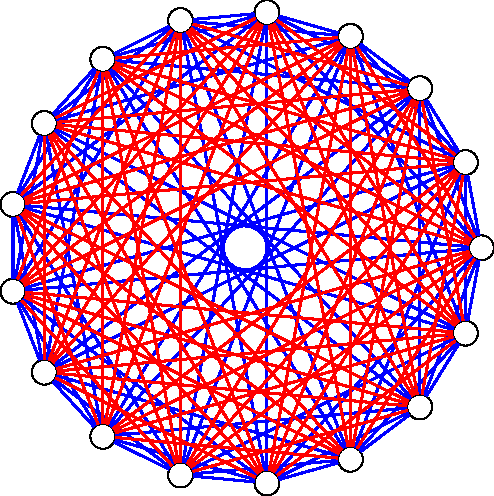
\includegraphics{figures/2_prelim_2_r44lb}
\caption{Coloração do $K_{17}$ sem $K_4$ monocromáticos.}
\label{prelim:fig:exr44}
\end{figure}
%%%%%%%%%%%%%%%%%%%%%%%%%%%%%%%%%%%%%%%%

%%%%%%%%%%%%%%%%%%%%%%%%%%%%%%%%%%%%%%%%
\begin{proposition}[Greenwood, Gleason~\cite{greenwood}]
\label{prelim:thm:exr44}
$R(4,4) > 17$.
\end{proposition}
%%%%%%%%%%%%%%%%%%%%%%%%%%%%%%%%%%%%%%%%
\begin{proof}
Vamos construir a coloração de arestas do grafo $G$ da Figura~\ref{prelim:fig:exr44}. Desta vez, trabalhamos no corpo $\Z{17}$, com $V(G) = \{v_0,\dots,v_{16}\}$. Definimos a seguinte relação em $\Z{17}$: dizemos que $i \sim j$ se $ i - j $ for um resíduo quadrático, isto é, se existe $x \in \Z{17}$ tal que $i - j \equiv x^2 \Mod{17}$.
Note que $i \sim j$ implica em $ j \sim i$ pois $-1 \equiv 4^2 \Mod{17}$. Temos também que $i \sim j$ implica em $i + k \sim j + k$ para todo $k$ e em $a^2 i \sim a^2 j$. Construímos a coloração $c$, então, da seguinte maneira:

\[c(v_i v_j) = \begin{cases}
  \text{vermelho}, & \text{se } i \sim j; \\
  \text{azul}, & \text{se } i \not\sim j.
\end{cases}\]

Agora, vamos mostrar que não existe $K_4$ monocromático em $G$. Suponha que $v_i, v_j, v_k, v_w$ formem um $K_4$ monocromático em $G$. Sem perda de generalidade, podemos supor $w = 0$ uma vez que esta relação é invariante à translações. Portanto, temos que os números $i$, $j$, $k$, $i - j$, $i - k$, $j - k$ são todos resíduos quadráticos ou são todos resíduos não-quadráticos. Suponha que todos eles sejam resíduos quadraticos. Como 17 é primo, $\Z{17}$ é um corpo, logo o elemento $i \neq 0$ possui inverso $i^{-1}$ e ele também é resíduo quadrático.
Definindo $a = i^{-1}j$, $b = i^{-1}k$, temos que os números $1$, $a$, $b$, $1 - a$, $1- b$, $a - b$ são todos resíduos quadráticos, uma vez que os resíduos quadráticos são fechados por multiplicação.

Se os números forem todos resíduos não-quadráticos, então $i^{-1}$ também é resíduo não-quadrático. Definindo $a$ e $b$ da mesma maneira, obtemos que os números $1$, $a$, $b$, $1 - a$, $1- b$, $a - b$ são todos resíduos quadráticos em $\Z{17}$.
Isto se deve ao fato de que em $\Z{p}$, com $p$ primo, o produto de dois resíduos não-quadráticos é um resíduo quadrático\footnote{Lembre o síbolo de Legendre, se $p$ é um primo ímpar e $a$ não é multiplo de $p$, definimos $\legendre{a}{p} = 1$ se $a$ é resíduo quadrático em $\Z{p}$ e $\legendre{a}{p} = -1$ caso contrário.
Como o símbolo de Legendre é uma função completamente multiplicativa, se $a$ e $b$ são resíduos não quadráticos, temos que $\legendre{ab}{p} = \legendre{a}{p} \legendre{b}{p} = (-1)(-1) = 1$, logo $ab$ é um resíduo quadrático. Veja mais no capítulo 5 do livro \emph{Introdução à Teoria dos Números} por José Plínio de Oliveira Santos~\cite{plinio}.}.

Em ambos os casos, temos que $1$, $a$, $b$, $1 - a$, $1- b$, $a - b$ são resíduos quadráticos em $\Z{17}$. Os resíduos quadráticos são 1, 2, 4, 8, 9, 13, 15 e 16, e não é possível escolher $a$ e $b$ de maneira que todos os números sejam simultaneamente resíduos. Isto pode ser verificado pelo raciocínio a seguir. Suponha que $a = 4$, então $1 - a \equiv 14 \Mod{17}$, que não é resíduo quadrático.
O mesmo verificamos se $a = 8$, $a = 13$ e $a = 15$, obtendo $1 - a \equiv 10 \Mod{17}$, $1 - a \equiv 5 \Mod{17}$ e $1 - a \equiv 3 \Mod{17}$ respectivamente, todos os casos não sendo resíduos quadráticos. Se $a = 9$ então $1 - a \equiv a \Mod{17}$ e os índices não são distintos.
Portanto, a única escolha restante é $a = 2$ e $b = 16$. Entretanto, $1 - a \equiv 16 \equiv b \Mod{17}$ e novamente não temos índices distintos.
\end{proof}
%%%%%%%%%%%%%%%%%%%%%%%%%%%%%%%%%%%%%%%%

%%%%%%%%%%%%%%%%%%%%%%%%%%%%%%%%%%%%%%%%
\begin{table}[ht!]
\small
\begin{tabular}{ll||llllllll}
& s & 3 & 4 & 5 & 6 & 7 & 8 & 9 & 10 \\
k &  &  &  &  &  &  &  &  &  \\ \hline \hline
3 &  & \texact{6} & \texact{9} & \texact{14} & \texact{18} & \texact{23} & \texact{28} & \texact{39} & \tbound{40}{42} \\ \hline
4 &  &  & \texact{18} & \texact{25} & \tbound{36}{41} & \tbound{49}{61} & \tbound{58}{84} & \tbound{73}{115} & \tbound{92}{149} \\ \hline
5 &  &  &  & \tbound{43}{49} & \tbound{58}{87} & \tbound{80}{143} & \tbound{101}{216} & \tbound{126}{316} & \tbound{144}{442} \\ \hline
6 &  &  &  &  & \tbound{102}{165} & \tbound{113}{298} & \tbound{132}{495} & \tbound{169}{780} & \tbound{179}{1171} \\ \hline
7 &  &  &  &  &  & \tbound{205}{540} & \tbound{217}{1031} & \tbound{241}{1713} & \tbound{289}{2826} \\ \hline
8 &  &  &  &  &  &  & \tbound{282}{1870} & \tbound{317}{3583} & \tbound{}{6090} \\ \hline
9 &  &  &  &  &  &  &  & \tbound{565}{6588} & \tbound{581}{12677} \\ \hline
10 &  &  &  &  &  &  &  &  & \tbound{798}{23556} \\ \hline
\end{tabular}
\centering
\caption{Valores e limitantes para $R(k,s)$ com $3 \leq k \leq s \leq 10$. }
\label{prelim:tab:ramsey}
\end{table}
%%%%%%%%%%%%%%%%%%%%%%%%%%%%%%%%%%%%%%%%

É natural, agora, tentar determinar $R(k,s)$ para outros valores de $k$ e $s$. No entanto, a dificuldade em determinar os valores de $R(k,s)$ cresce muito rapidamente com $s$ e $k$. Por exemplo, o valor de $R(5,5)$ não é conhecido e o valor de $R(4,5) = 25$ foi encontrado por uma busca computacional extensiva em 1995~\cite{rad45}. Existe um compêndio dinâmico dos resultados conhecidos sobre números de Ramsey pequenos, mantido por Radziszowski~\cite{small_ramsey}, os melhores valores conhecidos para $R(k,s)$ estão na Tabela~\ref{prelim:tab:ramsey}.

%%%%%%%%%%%%%%%%%%%%%%%%%%%%%%%%%%%%%%%%%%%%%%%%%%%%%%%%%%%%%%%%%%%%%%%%%%%%%%%%

\section{Limitantes Superiores}

Um fato interessante que podemos observar em todos os números que encontramos na seção anterior é que o argumento utilizado na prova do limitante superior é bem semelhante. De fato, podemos condensar esta idéia em um resultado à parte.

%%%%%%%%%%%%%%%%%%%%%%%%%%%%%%%%%%%%%%%%
\begin{theorem}[Greenwood, Gleason~\cite{greenwood}]
\label{prelim:thm:inequality}
$R(k,s) \leq R(k,s-1) + R(k-1,s)$.
\end{theorem}
%%%%%%%%%%%%%%%%%%%%%%%%%%%%%%%%%%%%%%%%
\begin{proof}
Sejam $G$ um grafo completo com $n$ vértices e $c$ uma RB-coloração. Suponha que não exista $K_k$ vermelho e nem $K_s$ azul. Seja $v \in V(G)$ um vértice qualquer. Consideramos as vizinhanças $N_R(v)$ e $N_B(v)$ de tamanhos $d_R(v)$ e $d_B(v)$, respectivamente. Assim, temos que $d_R(v) + d_B(v) = n-1$. Se $d_R(v) \geq R(k-1,s)$, então em $N_R(v)$ possui um $K_s$ azul ou um $K_{k-1}$ vermelho, que em conjunto com $v$ forma um $K_k$ vermelho, contradizendo nossa hipótese. Concluímos que $d_R(v) \leq R(k-1,s) - 1$. Similarmente, mostramos que $d_B(v) \leq R(k,s-1) - 1$. Portanto:
\begin{align*}
d_R(v) + d_B(v) &\leq R(k-1,s) + R(k,s-1) - 2 \\
n &\leq R(k-1,s) + R(k,s-1) - 1.
\end{align*}
Dessa maneira, escolhendo $n = R(k-1,s) + R(k,s-1)$ obtemos uma contradição, e portanto, concluímos que $G$ possui um $K_k$ vermelho ou um $K_s$ azul. Ou seja, $R(k,s) \leq R(k,s-1) + R(k-1,s)$, como queríamos.
\end{proof}
%%%%%%%%%%%%%%%%%%%%%%%%%%%%%%%%%%%%%%%%

Observe que desta resulta que $R(3,3) \leq R(2,3) + R(3,2) = 3 + 3 = 6$ e $R(4,4) \leq R(3,4) + R(4,3) = 18$. No entanto, ela não é justa para muitos valores de $k$ e $s$. Por exemplo, $R(3,4) \leq R(3,3) + R(2,4) = 10$. O argumento que foi utilizado para demonstrar que $R(3,4) \leq 9$ também pode ser generalizado na prosição seguir.

%%%%%%%%%%%%%%%%%%%%%%%%%%%%%%%%%%%%%%%%
\begin{theorem}[Greenwood, Gleason~\cite{greenwood}]
\label{prelim:thm:parity}
Se $R(k,s-1)$ e $R(k-1,s)$ forem pares, então
$R(k,s) < R(k,s-1) + R(k-1,s)$.
\end{theorem}
%%%%%%%%%%%%%%%%%%%%%%%%%%%%%%%%%%%%%%%%
\begin{proof}
Seja $R(k,s-1) = 2a$ e $R(k-1,s) = 2b$.
Sejam $G$ um grafo completo com $n = 2a + 2b -1$ vértices e $c$ uma RB-coloração. Suponha que não exista $K_k$ vermelho e nem $K_s$ azul. Fixe um vértice $v$ arbitrário. Seguindo o raciocínio da prova anterior, temos que $d_B(v) \leq 2a - 1$ e $d_R(v) \leq 2b - 1$. Como $d(v) = n - 1 = 2a + 2b - 2$, temos que $d_B(v) = 2a - 1$ e $d_R(v) = 2b - 1$. Isto vale para qualquer vértice $v$.
Consequentemente, os grafos $G_R$ e $G_B$ possuem uma quantidade ímpar de vértices de grau ímpar, o que é impossível pelo \emph{handshaking lemma}. Isto, então, contradiz a hipótese de que não existe $K_k$ vermelho e $K_s$ azul, concluindo que $R(k,s) \geq n = 2a + 2b -1$, o que finaliza a demonstração.
\end{proof}
%%%%%%%%%%%%%%%%%%%%%%%%%%%%%%%%%%%%%%%%

Esta proposição nos dá cotas ligeiramente mais precisas para alguns casos, por exemplo, chegamos em $R(3,4) \leq 9$. Outra consequência interessante da desigualdade do Teorema~\ref{prelim:thm:inequality} é um limitante superior genérico, que por sua vez nos permite obter uma versão ligeiramente melhor do Teorema~\ref{thm:intro:ramsey}.

%%%%%%%%%%%%%%%%%%%%%%%%%%%%%%%%%%%%%%%%
\begin{theorem}[Erdös, Szekerés~\cite{erdos_szekeres35}]
\label{thm:szekeres}
Para $k$ e $s$ inteiros positivos, temos:
\[R(k,s) \leq \binom{k + s - 2}{k - 1}\]
\end{theorem}
%%%%%%%%%%%%%%%%%%%%%%%%%%%%%%%%%%%%%%%%
\begin{proof}
Se $k = 1$ temos $R(1,s) = 1 = \binom{s - 1}{0}$. Se $k = 2$, temos $R(2,s) = s = \binom{s}{1}$. Procedemos agora por indução em $s + k$. Temos
\begin{align*}
  R(k,s) &\leq R(k,s-1) + R(k-1,s) \\
  &\leq \binom{k + s - 3}{k - 2} + \binom{k + s - 3}{k - 1} = \binom{k + s - 2}{k - 1}. \qedhere
\end{align*}
\end{proof}
%%%%%%%%%%%%%%%%%%%%%%%%%%%%%%%%%%%%%%%%

%%%%%%%%%%%%%%%%%%%%%%%%%%%%%%%%%%%%%%%%
\Needspace*{4\baselineskip}
\begin{corollary}[Erdös, Szekerés~\cite{erdos_szekeres35}]
\label{col:szekeres}
Para $k \to \infty$, temos
\[ \displaystyle R(k+1,k+1) \leq (1+o(1))\frac{4^k}{\sqrt{k \pi}}.\]
\end{corollary}
%%%%%%%%%%%%%%%%%%%%%%%%%%%%%%%%%%%%%%%%
\begin{proof}
Para transformar o limitante dado pelo Teorema~\ref{thm:szekeres} em um limitante assintótico para os números de Ramsey diagonais, vamos utilizar a aproximação de Stirling $n! = (1+o(1)) \sqrt{2n \pi} \left ( \frac{n}{e} \right)^n $, com $n \to \infty$, obtendo:
\begin{align*}
R(k+1,k+1) &\leq \binom{2k}{k} = \frac{(2k)!}{k!^2} = (1 +o(1)) \frac{\sqrt{4 k \pi} \left ( \frac{2k}{e} \right)^{2k} }{2k\pi \left ( \frac{k}{e} \right)^{2k} } \\
&= (1 +o(1))\frac{4^k}{\sqrt{k\pi}}. \qedhere
\end{align*}
\end{proof}
%%%%%%%%%%%%%%%%%%%%%%%%%%%%%%%%%%%%%%%%

Note que este limitante é ligeiramente melhor que o obtido no Teorema~\ref{thm:intro:ramsey} por causa da presença do termo $\sqrt{k}$ no denominador. Isto nos indica que os números de Ramsey diagonais crescem no máximo exponencialmente e com expoente estritamente menor que 4. Poucas melhoras substanciais neste limitante são conhecidas, sendo o melhor atual
\[R(k+1,k+1) \leq k^{-\alpha\frac{\log k}{\log \log k}} \binom{2k}{k},\]
para alguma constante $\alpha$ adequada, devido a David Conlon em 2009~\cite{conlon}. Note que o termo $k^{\alpha\frac{\log k}{\log \log k}}$ é subexponencial. Logo, este limitante não melhora a constante $4^k$ implicada pelo coeficiente binomial central $\binom{2k}{k}$.

%%%%%%%%%%%%%%%%%%%%%%%%%%%%%%%%%%%%%%%%%%%%%%%%%%%%%%%%%%%%%%%%%%%%%%%%%%%%%%%%

\section{Números de Ramsey multicoloridos}

Uma maneira muito natural de generalizar os números de Ramsey é considerar colorações de arestas com um número maior de cores. Estes números são conhecidos por \indef{números de Ramsey multicoloridos}.

%%%%%%%%%%%%%%%%%%%%%%%%%%%%%%%%%%%%%%%%
\begin{definition}
$R(t_1, \dots, t_k)$ é o menor inteiro positivo $n$ tal que qualquer coloração de arestas em $k$ cores do grafo $K_n$ possui, para algum $1 \leq i \leq k$, um $K_{t_i}$ da $i$-ésima cor.
\end{definition}
%%%%%%%%%%%%%%%%%%%%%%%%%%%%%%%%%%%%%%%%

Algumas observações são imediatas, por exemplo, se algum $t_i = 1$, então $R(t_1, \dots, t_k) = 1$, pois um $K_1$ é um $K_1$ de qualquer cor, em particular, da cor $C_i$. Se algum $t_i = 2$, digamos $t_k = 2$, então $R(t_1, \dots, t_{k-1}, 2) = R(t_1, \dots, t_{k-1})$, uma vez que um qualquer aresta da cor $C_i$ induz um $K_2$ desta cor. Além disso, os números de Ramsey possuem a seguinte simetria: se $\sigma$ é uma permutação de $\{1, \dots, k\}$, então
$R(t_{\sigma(1)}, \dots, t_{\sigma(k)}) = R(t_1, \dots, t_k)$.

Vamos ver que algumas propriedades dos números de Ramsey com duas cores podem ser estendidas para mais cores sem muito esforço. Por exemplo, em analogia ao Teorema~\ref{prelim:thm:inequality}, temos o resultado a seguir.

%%%%%%%%%%%%%%%%%%%%%%%%%%%%%%%%%%%%%%%%
\begin{theorem}[Greenwood, Gleason~\cite{greenwood}]
\label{prelim:thm:multi_inequality}
Para todos os inteiros positivos $t_i$, $1 \leq i \leq k$,
\[ R(t_1, \dots, t_k) \leq \sum_{i=1}^{k} R(t_1, \dots,t_{i-1}, t_i - 1, t_{i+1}, \dots, t_k) - k + 2. \]
\end{theorem}
%%%%%%%%%%%%%%%%%%%%%%%%%%%%%%%%%%%%%%%%
\begin{proof}
Sejam $G$ um grafo completo com $n$ vértices e $c$ uma $k$-coloração de arestas nas cores $C_1, \dots, C_k$. Suponha que não exista $K_{t_i}$ da cor $C_i$ para todo $1 \leq i \leq k$. Seja $v \in V(G)$ um vértice qualquer. Consideramos as vizinhanças $N_{C_i}(v)$, que possuem $d_{C_i}(v)$ vértices. Assim, temos que $\sum_{i=1}^{k} d_{C_i}(v) = n-1$.

Se $d_{C_i}(v) \geq R(t_1, \dots, t_i - 1, \dots, t_k)$ para algum $i$, então em $N_{C_i}(v)$ possui um $K_{t_i - 1}$ de cor $C_i$, pois $G$ não possui $K_{t_j}$ de cor $C_j$ para nenhum $j \neq i$. No entanto, unindo $v$ ao $K_{t_i - 1}$ de cor $C_i$ formamos um $K_{t_i}$ de cor $C_i$.
Contradizemos, então, nossa hipótese e temos que $d_{C_i}(v) \leq R(t_1, \dots, t_i - 1, \dots, t_k) - 1$ para todo $i$. Portanto,
\begin{align*}
n = \sum_{i=1}^{k} d_{C_i}(v)  + 1 \leq \sum_{i=1}^{k} R(t_1, \dots, t_i - 1, \dots, t_k) - k + 1.
\end{align*}
Dessa maneira, se um $K_n$ com uma $k$-coloração de arestas não possui $K_{t_i}$ da cor $C_i$, então $n \leq \sum_{i=1}^{k} R(t_1, \dots, t_i - 1, \dots, t_k) - k + 1$. Portanto, uma $k$-coloração de um grafo completo com $\sum_{i=1}^{k} R(t_1, \dots, t_i - 1, \dots, t_k) - k + 2$ vértices necessariamente possui algum $K_{t_i}$ de cor $C_i$, como queríamos demonstrar.
\end{proof}
%%%%%%%%%%%%%%%%%%%%%%%%%%%%%%%%%%%%%%%%

Analogamente ao Teorema~\ref{thm:szekeres}, transformamos a desigualdade deste teorema em um limitante com um coeficiente multinomial:

%%%%%%%%%%%%%%%%%%%%%%%%%%%%%%%%%%%%%%%%
\begin{corollary}[Greenwood, Gleason~\cite{greenwood}]
\label{prelim:thm:multinomial}
Para todos os inteiros positivos $t_i$, $1 \leq i \leq k$, temos:
\[ R(t_1 + 1, \dots, t_k + 1) \leq \binom{t_1 + \dots + t_k}{t_1, \dots, t_k} =  \frac{(t_1 + \dots + t_k)!}{t_1! \dots t_k!}. \]
\end{corollary}
%%%%%%%%%%%%%%%%%%%%%%%%%%%%%%%%%%%%%%%%

Podemos agora estimar o primeiro número multicolorido não-trivial (com todos os parâmetros maiores que 2), que é o $R(3,3,3)$. Utilizando o Teorema~\ref{prelim:thm:multi_inequality}, temos:
\begin{align*}
R(3,3,3) &\leq R(2,3,3) + R(3,2,3) + R(3,3,2) - 1 \\
&= 3R(3,3,2) - 1 = 3R(3,3) -1 = 17.
\end{align*}

De fato, temos que $R(3,3,3) = 17$. Para demonstrar este fato, precisamos construir uma 3-coloração de arestas de um $K_{16}$ sem que haja triângulos monocromáticos. Isto foi feito pela primeira vez por Greenwood e Gleason~\cite{greenwood}, mas, neste texto, vamos apresentar uma construção mais simples por Sun e Cohen~\cite{sun}.

%%%%%%%%%%%%%%%%%%%%%%%%%%%%%%%%%%%%%%%%
\begin{proposition}
\label{prelim:thm:exr333}
$R(3,3,3) > 16$.
\end{proposition}
%%%%%%%%%%%%%%%%%%%%%%%%%%%%%%%%%%%%%%%%
\begin{proof}
Vamos construir a coloração de arestas do grafo $G$ exibida na Figura~\ref{prelim:fig:exr333}. Desta vez, trabalhamos no corpo $\Z{2}^4 = \Z{2}\times\Z{2}\times\Z{2}\times\Z{2}$. Vamos particionar o conjunto dos elementos não nulos de $\Z{2}^4$ em três partes:
\begin{align*}
S_1&=\big\{ (1,1,0,0),\;(0,0,1,1),\;(1,0,0,1),\;(1,1,1,0),\;(1,0,0,0) \big\},\\
S_2&=\big\{ (1,0,1,0),\;(0,1,0,1),\;(0,1,1,0),\;(1,1,0,1),\;(0,1,0,0) \big\},\\
S_3&=\big\{ (0,0,0,1),\;(0,0,1,0),\;(0,1,1,1),\;(1,0,1,1),\;(1,1,1,1) \big\}.
\end{align*}

Cada uma destas partes $S_i$ possui a seguinte propriedade: se $a,b \in S_i$, então $a + b \not\in S_i$. Seja $V(G) = \{v_a : a \in \Z{2}^4\}$. Definimos a coloração de arestas $c$ em três cores da seguinte maneira:
\[c(v_a v_b) = \begin{cases}
  \text{vermelho}, & \text{se } a + b \in S_1; \\
  \text{azul}, & \text{se } a + b \in S_2; \\
  \text{verde}, & \text{se } a + b \in S_3.
\end{cases}\]

Esta coloração está bem definida pois os $S_i$ são disjuntos, cobrem todos os elementos não nulos de $\Z{2}^4$ e se $a,b \in \Z{2}^4$ com $a$ e $b$ distintos, então $a + b \neq 0$. De fato, dados $a$ e $b$ distintos, existe pelo menos uma coordenada em que eles diferem. Logo, esta coordenada será 1 na soma $a+b$, portanto $a + b \neq 0$.

%%%%%%%%%%%%%%%%%%%%%%%%%%%%%%%%%%%%%%%%
\begin{figure}[ht!]
\centering
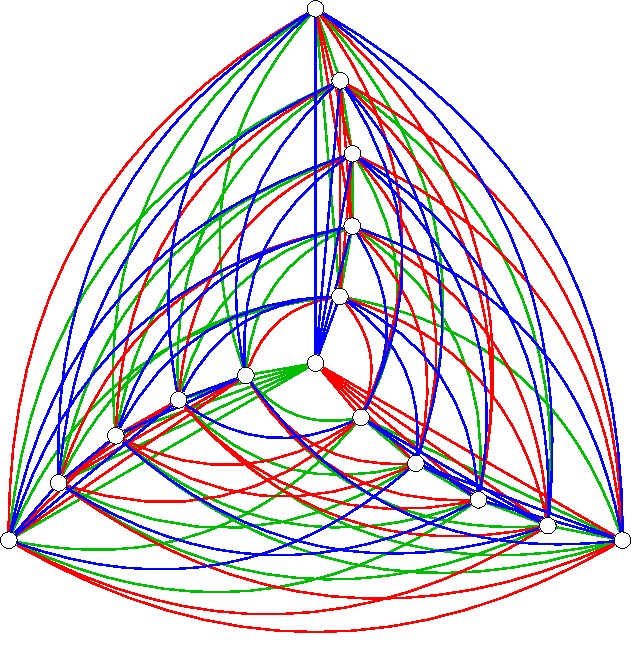
\includegraphics{figures/2_prelim_3_r333lb}
\caption{Coloração do $K_{16}$ em três cores sem $K_3$ monocromáticos.}
\label{prelim:fig:exr333}
\end{figure}
%%%%%%%%%%%%%%%%%%%%%%%%%%%%%%%%%%%%%%%%

Agora vamos ver que a coloração $c$ não possui triângulos monocromáticos.
Sejam $v_x, v_y, v_z$ os vértices de um triângulo qualquer. Suponha que duas das arestas sejam da mesma cor, digamos $c(v_x v_y) = c(v_x v_z)$. Vamos ver que a terceira aresta tem uma cor distinta. Temos para algum $i$, que $x + y, x + z \in S_i$. Utilizando a propriedade da soma de elementos de $S_i$,
temos que $(x+y) + (x+z) \not\in S_i$. Entretanto, $(x+y) +(x+z) = 2x + y + z = y + z$. Isto implica que $c(v_x,v_y)\neq c_(v_y,v_z)$. Portanto, $c$ não possui triângulos monocromáticos.
\end{proof}
%%%%%%%%%%%%%%%%%%%%%%%%%%%%%%%%%%%%%%%%

Uma coleção de números de Ramsey de bastante interesse é a dos números multicoloridos para triângulos. Denotamos por $R_r(3)$ o número de Ramsey $r$-colorido $R(3,3,\dots,3)$ com $r$ termos. De fato, já mostramos que $R_2(3) = 6$ e $R_3(3) = 17$. O número $R_4(3) = R(3,3,3,3)$ sabe-se que está entre 51 e 62. Em geral, temos as seguintes estimativas.

%%%%%%%%%%%%%%%%%%%%%%%%%%%%%%%%%%%%%%%%
\begin{theorem}
\label{prelim:thm:multi3ub} Para todo inteiro $r \geq 2$, $5^{r/2} \leq R_r(3) \leq 3 r!$.
\end{theorem}
%%%%%%%%%%%%%%%%%%%%%%%%%%%%%%%%%%%%%%%%
\begin{proof}
Para o limitante superior, aplicamos Teorema~\ref{prelim:thm:multi_inequality}, obtendo:
\begin{align*}
R_{r}(3) &\leq rR(3,\dots,3,2) = rR_{r-1}(3) \\
&\leq r(r-1)\dots3 R_2(3) = 3r!.
\end{align*}

Para o limitante inferior, faremos uma construção recursiva partindo da coloração da Figura~\ref{fig:intro:r33lb}. Suponha que $R_k(3) = n$. Considere o grafo completo $G$ com $5n$ vértices e cores $C_1, C_2, \dots, C_{k+2}$. Particione $V(G)$ em cinco partes com $n$ vértices: $S_1$, $S_2$, $S_3$, $S_4$ e $S_5$.
Podemos colorir as arestas dos subgrafos $G[S_i]$ com as cores $C_1, \dots, C_k$ de existam triângulos monocromáticos, uma vez que $R_k(3) \geq n$. As arestas que faltam colorir incidem em vértices $v_i \in S_i$ e $v_j \in S_j$ com $i \neq j$. Vamos colorir estas arestas nas cores remanescentes $C_{k+1}$ e $C_{k+2}$ utilizando o critério:
\[c(v_i v_j) = \begin{cases}
  C_{k+1}, & \text{se } i - j \equiv 1 \Mod{5} \\
  C_{k+2}, & \text{caso contrário}.
\end{cases}\]

%%%%%%%%%%%%%%%%%%%%%%%%%%%%%%%%%%%%%%%%
\begin{figure}[H]
\centering
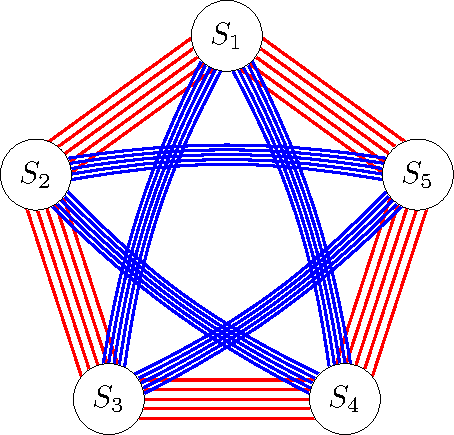
\includegraphics{figures/2_prelim_4_const}
\caption{Construção da coloração da Proposição~\ref{prelim:thm:multi3ub}.}
\label{prelim:fig:const}
\end{figure}
%%%%%%%%%%%%%%%%%%%%%%%%%%%%%%%%%%%%%%%%


A Figura~\ref{prelim:fig:const} exemplifica esta construção. Note que $c$ não possui triângulo monocromático nas cores $C_1, \dots, C_k$, uma vez que construímos a coloração em $G[S_i]$ desta maneira. Além disso, $c$ também não possui triângulo monocromático nas cores $C_{k+1}$ e $C_{k+2}$ por construção.

Desta forma, concluimos que existe uma $k+2$-coloração de arestas de $G$ sem triângulo monocromático. Logo $R_{k+2}(3) \geq 5n = 5R_k(3)$. Aplicando esta relação repetidamente, obtemos:
\begin{align*}
R_{2k}(3) &\geq 5^{k-1}R_2(3) = 5^{k-1}\cdot6 \geq 5^{k}  \\
R_{2k+1}(3) &\geq 5^{k-1}R_3(3) = 5^{k-1}\cdot17 = 5^k \left(\frac{17}{5}\right) \geq 5^{k + 1/2}
\end{align*}
Em qualquer caso, obtemos $R_{r}(3) \geq 5^{r/2}$.
\end{proof}
%%%%%%%%%%%%%%%%%%%%%%%%%%%%%%%%%%%%%%%%

Embora os limitantes encontrados no Teorema~\ref{prelim:thm:multi3ub} não sejam os melhores conhecidos, eles estão próximos. Note que existe uma diferença bem grande em ordem entre $5^{r/2}$ e $3r!$ com $r \to \infty$. Mesmo assim, sabe-se que o  limite
\[ \lim_{r \to \infty} \left(R_r(3) \right)^{1/r} \]
existe~\cite{chung1983survey}, embora possa ser infinito. O Teorema~\ref{prelim:thm:multi3ub} mostra que este limite é pelo menos $\sqrt{5} \approx 2.236$.
Não se sabe muito mais sobre os números $R_r(3)$. Para o caso $r=4$, por exemplo, os melhores limitantes conhecidos são $R_4(3) \geq 51$~\cite{chung1973ramsey} e $R_4(3) \leq 62$~\cite{fettes2004upper}.

%%%%%%%%%%%%%%%%%%%%%%%%%%%%%%%%%%%%%%%%%%%%%%%%%%%%%%%%%%%%%%%%%%%%%%%%%%%%%%%%


%%%%%%%%%%%%%%%%%%%%%%%%%%%%%%%%%%%%%%%%%%%%%%%%%%%%%%%%%%%%%%%%%%%%%%%%%%%%%%%%
